\chapter{Real-Time Conditioned Media Assay}
\label{App:RealTimeCM}

\section{Passive Methods for Producing Slow Flow in Microchannels} \label{chap:slowFlow}

Perfusion culture is a major form of culture in microfluidic devices. However, perfusion typically requires active pumping methods such as the use of syringe pumps to produce the flow. Use of such technology often requires microfluidic devices to be multiplexed where the flow in multiple culture chambers is driven by a single pump, reducing the ability to compartmentalize culture experiments. The devices designed and implemented in this set of experiments are aimed at producing slow perfusion rates (\ie , nL/hr). The rates of perfusion we intend to use are interesting for multiple reasons. The flow rate is on the order of diffusion rates. Using only changes in channel geometry, the \me\ of the cell can be transformed from being dominated by convection to being dominated by diffusion. This affords us the ability to create \me s in which we can replenish media without creating significant gradients in concentrations. Further, we can utilize the convection dominant environments to bias signaling between two culture chambers, opening the door to new assays in which we can easily modulate the soluble factor signaling between different cell types.

The fact that these slow perfusion devices do not require tubes means that each perfusion assay can remain independent, instead of be linked or multiplexed. Keeping the assays independent allows for easier transition into higher throughput experimentation, a long-term goal for our platform. The devices can also be operated using a standard micro-pipette, which helps to increase the accessibility of the method and encourages development new experimental designs.

There are two significantly different methods by which we propose to produce slow flow, via evaporation and via manipulation of surface tension using surfactants. Preliminary data has been collected for evaporation driven flow and has been successfully implemented but would benefit from refinement. The devices developed in this section will be evaluated for their repeatability and ease of use. One of the designs will be selected for advancement into the next two sets of experiments. \emph{Since a proof-of-concept has been validated using evaporation driven flow, there is at least one viable option as we move forward and begin performing perfusion culture experiments.}

\subsection{Device Designs}\label{sec:deviceDesign}
\subsubsection{Evaporation}\label{sec:deviceDesignEvap}
The basic device design consists of a port at which evaporation is allowed to drive volume loss that is connected to possibly many other ports where evaporation is kept to a minimum. Therefore, the flow that occurs through the device is dictated by the volume loss at the evaporation port. Furthermore, the control of that flow rate depends upon controlling the rate of evaporation. The rate of evaporation is generally controlled by manipulating the relative humidity over the evaporation port. There are many ways to control relative humidity, some of which are pursued here and diagramed in Fig \ref{fig:evaporationDevices}.

\begin{figure}[!ht]
\centering
a) 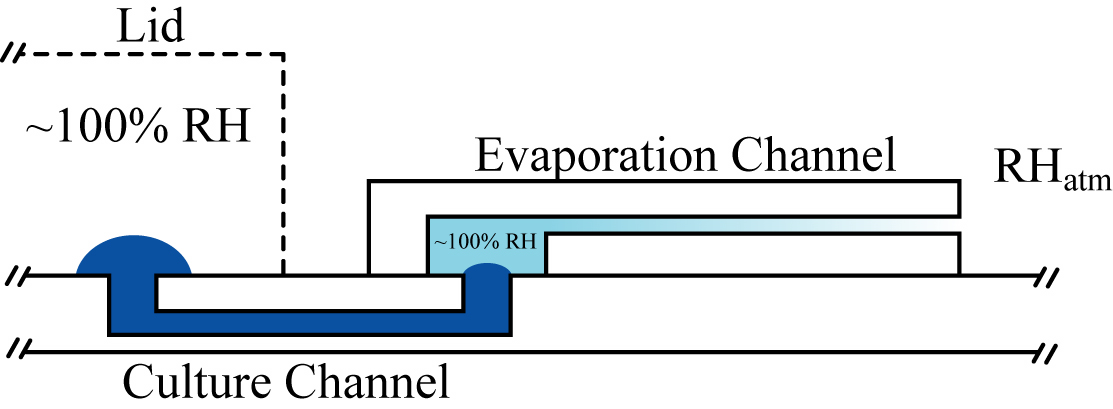
\includegraphics[width=4.5in]{EvaporationChannel.jpg}


\vspace{0.5cm}


b) 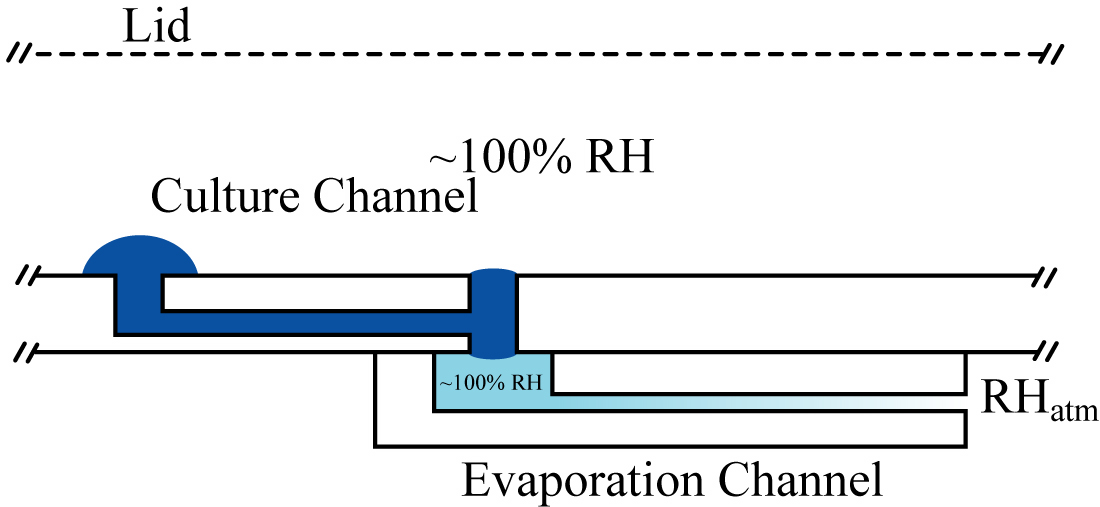
\includegraphics[width=4.5in]{EvaporationChannel2.jpg}
\caption{\textbf{Schematic representation of two different methods for controlling humidity to drive slow flow via evaporation}. The device design minimizes evaporation at non-evaporation ports (\ie , the port on the left) while the evaporation channel is an empty microchannel that resists evaporation at a rate proportional to the ratio of length to cross-sectional area. Varying the length of the evaporation channel linearly varies the evaporation rate and thus the flow through the device. a) Method 1 - Top-Side Evaporation Channel:  Both ports of the device are on the top-side of the substrate. b) Method 2 - Bottom-Side Evaporation Channel:  The evaporation channel is situated on the bottom-side of the substrate by creating a hole through the substrate. Preliminary results suggest the bottom-side design has advantages with respect to sterilization procedures, ease of use, and compatibility with PDMS and a material for making the microchannels.}
%Method 1) Two chamber design with variable sacrificial fluid. The inner chamber attempts to minimize evaporation from the non-evaporation ports while the exterior chamber controls evaporation through an appropriate amount and placement of sacrificial fluid (empirically determined) [CITE JAY/ERWIN].
\label{fig:evaporationDevices}
\end{figure}

The two designs implement the use of an evaporation vent. The evaporation vent is a microchannel that is left unfilled. One end of the channel has a port that encloses the evaporation port of the perfusion device. Vapor that is diffusing away from the evaporation port must diffuse through the evaporation vent. Therefore, the flux of vapor from the evaporation vent can be controlled by designing the cross-sectional area and length of the channel resist evaporation appropriately for the external humidity conditions. The resistance of the evaporation vent to vapor diffusion is proportional to the ratio of its length to its cross-sectional area. Silica beads will be used to control the external humidity at the underside of the device. 

%The major advantage using the evaporation vent is that the humidity external to the device does not need to be controlled such as with the use of a standard cell culture incubator. This makes the device much more portable and robust to external changes in humidity. If the evaporation vent is designed for dry external environments, then the device will better suited for the environments typical of microscopes or culture hoods, also it could eliminate the requirement for a humidified culture incubator. 

As this method is intended for use in cell culture, one obstacle to the implementation of an evaporation driven method for flow is the accumulation of solute near the evaporation port. Over the time-course of evaporation, increased osmolarity or high concentrations of toxic factors, if allowed to reach the culture region of the device, could adversely effect results. A diffusion valve that was developed in previous work with Erwin Berthier and used in previous work by lab members \cite{Frisk:2008pi} will be used to keep accumulation of solute from diffusing into regions used for cell culture. The diffusion valve is a microchannel with cross-sectional area to length ratio such that when a predetermined flow rate exists through the valve, solute, including small molecules such as ions, cannot diffuse significantly upstream. Thus, given two chambers connected by a diffusion valve, the upstream chamber is diffusionally isolated from the downstream chamber. 

Fig \ref{fig:pecletFlow} shows a plot of normalized concentration versus normalized length within the diffusion valve region given flows of various characteristic Peclet numbers. The Peclet number describes the balance between convective and diffusive transport given a fluid velocity, characteristic length, and diffusion coefficient (Pe = $L\,v/D$). The characteristic length that is appropriate for the diffusion valve is the valve length, as we are interested in transport along the length of the channel. Peclet numbers of ~3.0 suggest that, at stead-state, the upstream chamber is at 5\% the concentration of the downstream chamber. Some similar calculations include $\sim$4.6 $\rightarrow$ 1\%, $\sim$10 $\rightarrow$ 0.004\%, and $\sim$15 $\rightarrow$ 0.00003\%. It may seem extreme to look at such high values of the Peclet but many soluble factors can illicit cellular responses over many orders of magnitude of concentration. However, the calculations suggest that the upstream chamber can be effectively isolated from the downstream chambers.

A more detailed treatment of the diffusion valve including governing equations is contained in the Appendix.

\begin{figure}[!ht]
\centering
\includegraphics[width=3.5in]{DiffusionValve.pdf}
\caption{\textbf{Diffusion valve operation}. Plot of normalized concentration ratio (concentration at position $x/L$ divided by concentration at inlet of the downstream chamber) for various values of the Peclet number for the diffusion valve. $x/L=0$ is at the downstream chamber and $x/L=1$ is at the upstream chamber.}
\label{fig:pecletFlow}
\end{figure}

Another important consideration in the design of slow flow methods such as this is the range of appropriate flow rates for any attached culture chambers. The goal of future work is to create slow perfusion flow without significantly affecting the diffusive transport of factors locally within each culture chamber. Just as the diffusion analysis of Fig \ref{fig:pecletFlow} applies to the diffusion valve, it also applies to the culture chambers. Therefore, a desirable situation would be to keep the Peclet number below a value of 1 in the culture chamber, thereby attempting to minimize the gradient of factors that exist in the culture chamber. The diffusion valve is aimed at isolating small molecules while the culture chambers are aimed at evenly distributing large molecules. This disparity is accounted for in the designing of the relative lengths and widths of the culture chambers and diffusion valves. If the Peclet number is too high in the culture chamber, the cross-sectional area of the culture chamber can be increased or the chamber length can be reduced or, if it easier to modify the diffusion valve, the diffusion valve could be reduced in cross-sectional area or lengthened. These changes in dimensions allow the user to design chambers and valves to the particular flow or media exchange rate that is desired for culture chamber. Thus, fluid exchange rates can be adjusted to increase or decrease overall levels of accumulating factor and still maintain relatively even distributions of factor within the chamber.

The design parameters of the evaporation-based device are listed in Tab \ref{tab:evaporation}.

\begin{table}[!ht]
\centering
\begin{tabular}{ll} \toprule
Parameter & Decription \cr \midrule
$D_{d}$ & {\underline D}iffusion coefficient of solute of interest in the {\underline d}iffusion valve \cr
$D_{c}$ & {\underline D}iffusion coefficient of solute of interest in the {\underline c}ulture chamber \cr
$L_{d}$ & {\underline L}ength of the {\underline d}iffusion valve \cr
$L_{c}$ & {\underline L}ength of the {\underline c}ulture chamber \cr
$L_{e}$ & {\underline L}ength of the {\underline e}vaporation vent \cr
$A_{d}$ & Cross-sectional {\underline a}rea of the {\underline d}iffusion valve \cr
$A_{c}$ & Cross-sectional {\underline a}rea of the {\underline c}ulture chamber \cr
$A_{e}$ & Cross-sectional {\underline a}rea of the {\underline e}vaporation vent \cr
$RH$ & The {\underline r}elative {\underline h}umidity external to the device \cr \bottomrule
\end{tabular}
\caption{\textbf{Table of design parameters for evaporation mediated slow flow device}.}
\label{tab:evaporation}
\end{table}

\subsubsection{Surfactant Mediated Flow}\label{sec:deviceDesignSurf}
Just as surface tension plays the dominant role in producing flow via traditional \pp , surface tension can be modified to produce flow without any addition of fluid. In this device, surfactant is delivered to the output port of the device to cause a change in surface tension resulting in a pressure change that then causes flow in the perfusion device. Our chosen method of surfactant delivery is diffusion through a microchannel. Therefore, the time-scales of the flow are limited by diffusion and can be many hours, as dictated by the geometry of the delivery channel and reservoirs. The total volume pumped via this method is limited by the volumes of the input and output drop of the channel that is being influenced. The fluid velocity within the channel will be a result of the diffusion kinetics, the droplet sizes, and finally the channel geometry. One advantage of this design is that the volumes pumped are small and the fluid flow rate is limited by diffusion, therefore, very slow flow rates can be achieved in a controlled manner. A schematic of the device is shown in Fig \ref{fig:surfactantDevices}.

\begin{figure}[!ht]
\centering
\includegraphics[width=5in]{SurfactantFlowDiagram.pdf}
\caption{\textbf{Slow flow via surfactant diffusion}. Schematic representation of slow perfusion device mediated by controlled delivery of surfactants. Diffusion of surfactant reduces surface tension at the affected output drop. The reduced surface tension causes fluid to flow towards the affected output drop from other input ports in amounts related to the input port radii. Inputs with larger radii will be larger sources of flow. The diffusion valve can be designed to isolate the surfactant from upstream culture areas.}
\label{fig:surfactantDevices}
\end{figure}

The slow flow device shown in Fig \ref{fig:surfactantDevices}, is designed to validate the surfactant-based slow flow method and is not intended for culture. One or multiple culture chambers and their associated ports can be included upstream of the diffusion valve, which is in place to isolate surfactant from the culture components. As mentioned earlier, the diffusion valve is very effective at minimizing diffusion upstream for flows with a Peclet number significantly greater than 1. The output port is connected to a surfactant delivery channel and port. When very small volume of containing a high concentration of surfactant is placed at the surfactant delivery port, negligible flow will occur from \pp\ as the surfactant delivery port has a very small radius. The surfactant will then diffuse through the surfactant delivery channel to affect the output drop. Surfactant diffusing into the output drop will cause a reduction in surface tension and pressure. The loss of pressure causes flow towards the output drop, thereby producing flow for the diffusion valve to isolate surfactant from any upstream culture components.

%Specific dimensions were chosen via simulation of the device in Matlab using 1D simplified models of diffusion in the microchannel. The model assumes even mixing in the output port and a linear relationship between surfactant concentration and surface tension. The model was simulated for a range of surface tensions that would produce a $\sim$70\% reduction in surface tension at the output port (see Appendix). 

Initial simulations suggest that the diffusion process can be made to last hours or days with appropriate geometries. Over those time-courses, input and output volumes can be chosen to result in flow rates that would result in exchange of culture chamber media from fractions per day up to many times per day suggesting that it would be an appropriate method for slow perfusion microchannel culture.

Design parameters of the device, when used to perfuse fluid through a culture chamber are very similar to the evaporation based device with slight differences as shown in Tab \ref{tab:surfactant}.

\begin{table}[!ht]
\centering
\begin{tabular}{ll} \toprule
Parameter & Decription \cr \midrule
$D_{d}$ & {\underline D}iffusion coefficient of solute of interest in the {\underline d}iffusion valve \cr
$D_{c}$ & {\underline D}iffusion coefficient of solute of interest in the {\underline c}ulture chamber \cr
$D_{s}$ & {\underline D}iffusion coefficient of {\underline s}urfactant \cr
$L_{d}$ & {\underline L}ength of the {\underline d}iffusion valve \cr
$L_{c}$ & {\underline L}ength of the {\underline c}ulture chamber \cr
$L_{s}$ & {\underline L}ength of the {\underline s}urfactant delivery channel \cr
$A_{d}$ & Cross-sectional {\underline a}rea of the {\underline d}iffusion valve \cr
$A_{c}$ & Cross-sectional {\underline a}rea of the {\underline c}ulture chamber \cr
$A_{s}$ & Cross-sectional {\underline a}rea of the {\underline s}urfactant delivery channel \cr
$S$ & The type of {\underline s}urfactant delivered \cr \bottomrule
\end{tabular}
\caption{\textbf{Table of design parameters for surfactant mediated slow flow device}.}
\label{tab:surfactant}
\end{table}

One important unknown aspect of the design suggested by the parameter $S$ in Tab \ref{tab:surfactant} is the identity of the surfactant and the effectiveness of the surfactant to reduce surface tension in the media. A preliminary experiment will be performed using a goniometer to determine the surface tension profile of different concentrations of surfactant and media. The profile will influence the flow rate progression over time and will be important to evaluating the ability of this method to produce consistent flow over long intervals. One surfactant of interest is bovine serum albumin (BSA).

\subsection{Methods}

Methods common to many pieces of the work proposed here are described in the Appendix such as device manufacture and modeling of diffusion, signaling, and response.

\subsubsection{Device Characterization}
The device designs will be characterized by measuring total flow over time and observing the quasi-steady-state convection-diffusion of dye or fluorescently labeled molecules at different times. In the case of the evaporation-based slow flow device, flow will be measured as the total volume loss over time compared to a `no evaporation' control, whereas in the case of the surfactant mediated flow device, droplet profile will be measured at the input port to infer volume at various time-points and will also be compared to a `no evaporation' control.

\subsection{Preliminary Results} \label{sec:prelimCCResults}

Some preliminary testing has already been accomplished with respect to slow-perfusion via evaporation. However, the results were obtained in the context of work towards a `one-way co-culture' device and thus diagrams show devices that have two chambers instead of one as suggested in section \ref{sec:deviceDesignEvap}. Fig \ref{fig:oneWayDye}a shows images of a slow-perfusion device with two culture chambers. Each image shows a different scenario. The bright-field image is intended to show the shape of the device. The balloons labeled with the word `add' indicate that fluorescent dye was added to the chamber prior to flow. The images with the square chambers are simulation results false colored like the dye. In each case, the dye in the experiment and simulation are confined to be at or below the chamber to which it was added over the course of 24 hours. Thus, evaporation was successfully implemented to direct a slow flow that transports fluid at similar rates to diffusion in the culture chambers and the diffusion valves were effective barriers to diffusion upstream. The fluid velocity simulation diagram of Fig \ref{fig:oneWayDye} indicates the relative flow rates that exist in the diffusion valves versus the chambers.

\begin{figure}[!ht]
\begin{center}
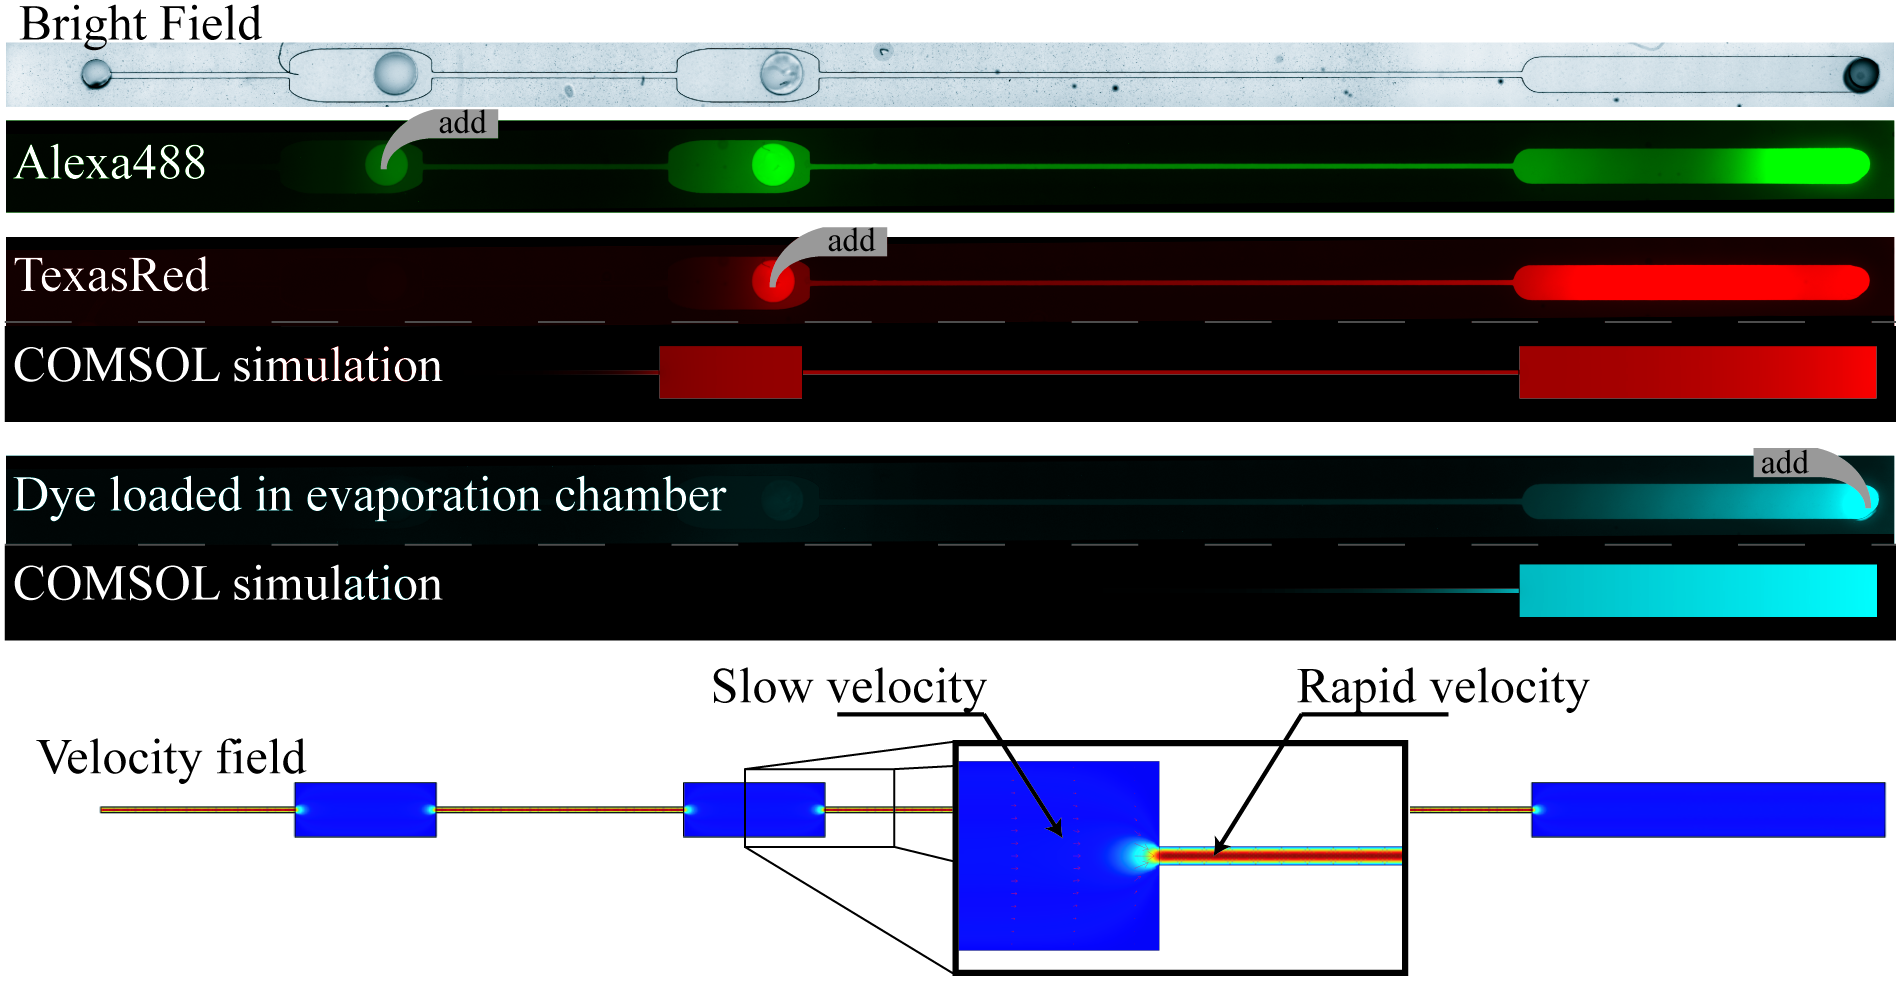
\includegraphics[width=6.5in]{OneWay_Illustration_figure.png}
\caption{\textbf{Preliminary validation of real-time conditioned media assay device operation}. Microscope images demonstrating the function of the diffusion valve. Different dyes (Alexa488 and TexasRed bound to Dextran 10kD) were loaded in the chambers destined for cell culture and imaged after 24 hours. The profiles show the presence of dyes downstream of diffusion valves but not upstream. COMSOL simulations were performed by supposing constant production of dye in the chamber after 20 hours. The velocity fields obtained are displayed.}
\label{fig:oneWayDye}
\end{center}
\end{figure}

\subsection{Expected Challenges}
Preliminary results suggest that there will be some challenges with respect to the technical implementation. One of the evaporation designs requires cutting through the polystyrene substrate, which can be a challenge. However, we have just purchased a CO$_{2}$ laser cutting system which has the capability to cut holes through polystyrene with sufficient accuracy. Processing parameters for optimal hole manufacture are still undetermined but is the focus of a hired undergraduate over the semester.

Further, the evaporation device that requires laser cutting will also need a method to create a dry environment on the bottom side of the device. Preliminary tests have shown that we can either use a sealed lid and a dry incubator or a non-sealed lid and a sealed chamber under the channel in which humidity is depleted using silica beads. The latter appears to have the most advantages as it allows for a more free gas exchange with the gas controlled incubator. However, the capacity of the silica beads to maintain a dry environment has not been thoroughly investigated but first indications are that they are quite sufficient.

\paragraph{Side note for future work:}Just as silica beads can be used to create an atmosphere depleted of water vapor at the underside of the evaporation device, other materials exist that can deplete or supply other gaseous molecules such as oxygen. In this way, different concentrations of gaseous molecules could be maintained at each end of a microchannel to create gradients. The work proposed here represents a first step towards such gradient devices that could be a way to readily examine the effects of microenvironmental parameters such as oxygen tension.

\section{Cross Flow in the Diffusion Region}
The following fluidic device can be analyzed using an electrical analogy (see Fig \ref{App:PerfusionCulture:fig:device}). The electric circuit analogy can be split into an analogous circuit in which there are two voltage sources. Now the problem can be solved using superposition. When using superposition, one voltage source is disconnected and the circuit is solved. The same is done using the other as the sole voltage source. This solutions are then added to obtain total voltages and currents which should match the results of the original circuit. 

\begin{figure}[!ht]
\centering
a) \includegraphics[height=2in]{Device.pdf}     b) \includegraphics[height=2in]{Original.pdf}
\caption{\textbf{Perfusion co-culture}. Perfusion co-culture device in which flow ratios will be estimated and its electric circuit analog.}
\label{App:PerfusionCulture:fig:device}
\end{figure}

Fig \ref{fig:circuit} shows two circuits, that when solved and their solutions added together, give the solution to the original circuit shown in Fig \ref{App:PerfusionCulture:fig:device}.

\begin{figure}[!ht]
\centering
\includegraphics[height=2in]{Analog.pdf}
\caption{\textbf{Perfusion co-culture circuit analog}. Diagrams of circuits that when added together, are equivalent to the original circuit of Fig \ref{App:PerfusionCulture:fig:device}. The circuits shown here are easier to solve and are used in the math that follows to find the ratios of currents or fluid flows through the device as compared to the total flow through the device.}
\label{fig:circuit}
\end{figure}

The left-hand and right-hand circuit have the following equivalent resistances.

\begin{equation}
R_{LH} = R_{1} + \frac{1}{\frac{1}{R_{4}} + \frac{1}{C_{LH}}}\textrm{, where } C_{LH} = R_{3} + \frac{1}{\frac{1}{R_{5}} + \frac{1}{R_{2}}}
\end{equation}
\begin{equation}
R_{RH} = R_{2} + \frac{1}{\frac{1}{R_{5}} + \frac{1}{C_{RH}}} \textrm{, where } C_{RH} = R_{3} + \frac{1}{\frac{1}{R_{4}} + \frac{1}{R_{1}}}
\end{equation}

Therefore the ratio $I_{1}/I_{2}$ is equal to the ratio $R_{RH}/R_{LH}$. Now if we solve for $I_{3}$ in each circuit, we can use the information to indicate the proporation of total current through the circuit that is devoted to pass through $R_{3}$ (\ie , the fluid flow through the diffusion valve).

In the left-hand circuit, 
\begin{equation}
I_{2}^{LH} =\frac{V}{R_{LH}}
\end{equation}
\begin{equation}
I_{3}^{LH} =\frac{I_{1}^{LH}}{1+ \frac{C_{LH}}{R4}}
\label{equ:LHI3}
\end{equation}
\begin{equation}
I_{2}^{LH} =\frac{I_{3}^{LH}}{1+\frac{R_{2}}{R_{5}}}
\end{equation}
and in the right-hand circuit
\begin{equation}
I_{1}^{RH} =\frac{V}{R_{RH}}
\end{equation}
\begin{equation}
I_{3}^{RH} =\frac{I_{1}^{RH}}{1+ \frac{C_{RH}}{R5}}
\label{equ:LHI3b}
\end{equation}
\begin{equation}
I_{1}^{RH} =\frac{I_{3}^{RH}}{1+\frac{R_{1}}{R_{4}}}
\end{equation}
and by superposition,
\begin{equation}
I_{3} = I_{3}^{LH} - I_{3}^{RH}
\label{equ:I3}
\end{equation}
\begin{equation}
I_{1} = I_{1}^{LH} - I_{1}^{RH}
\label{equ:I1}
\end{equation}
\begin{equation}
I_{2} = I_{2}^{RH} - I_{2}^{LH}
\label{equ:I2}
\end{equation}

The minus sign is to indicate that the $I_{1}$, $I_{2}$, and $I_{3}$ currents are in opposite directions in the RH and LH circuits. This then allows us to write the proportion of total current that flows through the diffusion region as the following.

\begin{equation}
\textrm{Cross Flow Ratio} = \frac{I_{3, tot}}{I_{1} + I_{2}}
\end{equation}

Using the above equations Fig \ref{fig:crossFlow} was created to observe the influence of unbalanced resistance on the rate of cross flow through the bridge relative to the total flow through the device. This is done by varying only the resistance of $R_{5}$.

\begin{figure}[!ht]
\centering
\includegraphics[width=3.5in]{CrossFlowPlot.pdf}
\caption{\textbf{Cross-flow during perfusion co-culture}. Calculations of relative cross flow rate using electrical analog equations for different output resistance ratios.}
\label{fig:crossFlow}
\end{figure}

\section{Peclet Ratio}

Diffusive flux in a rectangular duct with 1D diffusion is proportional to the following expression, $J \propto D\,A/L$ where $D$ is the diffusion coefficient describing the solvent and solute, $A$ is the cross-sectional area of the duct, and $L$ is the length of the duct. Therefore, to maximize the flux through the diffusion region we would like to maximize $A$ and minimize $L$.

In order to maximize diffusive flux in the parallel perfusion co-culture device the diffusion region length, $h_{d}$, will likely be the same height as the culture region, $h_{c}$, and the length roughly 1/10$^{th}$ the culture chamber length (\ie , $h_{d}/h_{c} \approx 1$, and $L_{d}/L_{c} \approx 0.1$). A significant width for the diffusion region might also be roughly the width of the culture chambers (\ie , $w_{d}/w_{c} \approx 1$).

The Peclet number of a flow is given by $Pe = L\,v/D$ which can also be written in terms of the flow rate for a duct as $Pe = L\, Q \, w \, h/D$. Further, if we estimate the flow rate in each culture chamber as being half of the total flow for a reasonably balanced system, we can write an expression for the ratio of Peclet numbers for the culture chambers versus the diffusion region between the chambers ($Pe_{c}/Pe_{d}$, culture chamber over diffusion region).

\begin{equation}
Pe_{c}/Pe_{d} = \frac{L_{c}Q_{c}w_{c}h_{c}}{L_{d}Q_{d}w_{d}h_{d}}
\end{equation}

Using conclusions from the previous section and assuming the flow in each culture chamber is about half of the total flow through the device, we can estimate the flow rate ratios, $Q_{c}/Q_{d} \approx 0.04$. We have already suggested that $h_{c}/h_{d} \approx 1$, $w_{d}/w_{c} \approx 1$, and $L_{c}/L_{d} \approx 0.1$. Therefore, it is expected that the ratio of the diffusion region Peclet number and culture chamber peclet number will be roughly $0.04 \times 1 \times 1 \times 0.1 \approx 0.004$. Since the aim of the coculture device is to keep the Peclet number in the culture chamber close to 1, the Peclet number in the diffusion region will be $\ll 1$ ensuring relatively unbiased communication between the two chambers.


%Now if we assume the following,
%\begin{equation}
%R1/R2 = \alpha
%\end{equation}
%\begin{equation}
%R4/R5 = \beta
%\end{equation}
%then each of the above equations can be collapsed to the following.

%\begin{equation}
%R_{LH} = \alpha R_{2} + \frac{1}{\frac{1}{\beta R_{5}} + \frac{1}{C_{LH}}}\textrm{, where } C_{LH} = R_{3} + \frac{1}{\frac{1}{R_{5}} + \frac{1}{R_{2}}}
%\end{equation}
%\begin{equation}
%R_{RH} = R_{2} + \frac{1}{\frac{1}{R_{5}} + \frac{1}{C_{RH}}} \textrm{, where } C_{RH} = R_{3} + \frac{1}{\frac{1}{\beta R_{5}} + \frac{1}{\alpha R_{2}}}
%\end{equation}



%		Clh = (R3 + (1/((1/R5) + (1/R2))));
%		System.out.println("Clh: " + Clh);
%		Crh = (R3 + (1/((1/R4) + (1/R1))));
%		System.out.println("Crh: " + Crh);
%		
%		Rlh = R1 + 1/((1/R4) + (1/Clh));
%		System.out.println("Rlh: " + Rlh);
%		Rrh = R2 + 1/((1/R5) + (1/Crh));
%		System.out.println("Rrh: " + Rrh);
%		
%		I1lh = 1/Rlh;
%		System.out.println("I1lh: " + I1lh);
%		I3lh = I1lh/(1+(Clh/R4));
%		System.out.println("I3lh: " + I3lh);
%		I2lh = I3lh/(1+(R2/R5));
%		System.out.println("I2lh: " + I2lh);
%		
%		I2rh = 1/Rrh;
%		System.out.println("I2rh: " + I2rh);
%		I3rh = I2rh/(1+(Crh/R5));
%		System.out.println("I3rh: " + I3rh);
%		I1rh = I3rh/(1+(R1/R4));
%		System.out.println("I1rh: " + I1rh);








